\begin{flushleft}
Per poter costruire una tabella abbiamo scritto il seguente codice MatLab (lo script usa function definite a parte che è possibile vedere a pagina \pageref{functcap2}):
\lstinputlisting[language=Matlab]{cap_2/es6/es6.m}
Sotto forma tabellare rappresentiamo il numero di iterazioni effettuate dai 3 algoritmi (salvate nella matrice $iter$):

\begin{center}
\begin{tabular}{|c|c|c|c|}
\hline
$tol_x$ & Newton & Secanti & Corde \\
\hline
$10^{-1}$ & 2 & 3 & 2 \\
$10^{-2}$ & 3 & 3 & 8 \\
$10^{-3}$ & 3 & 4 & 15 \\
$10^{-4}$ & 3 & 5 & 22 \\
$10^{-5}$ & 4 & 5 & 28 \\
$10^{-6}$ & 4 & 5 & 35 \\
$10^{-7}$ & 4 & 5 & 42 \\
$10^{-8}$ & 4 & 6 & 48 \\
$10^{-9}$ & 4 & 6 & 55 \\
$10^{-10}$ & 5 & 6 & 62 \\
\hline
\end{tabular}
\end{center}
Questo risultato è possibile vederlo tramite il plot MatLab:
\begin{figure}[H]
\label{fes26}
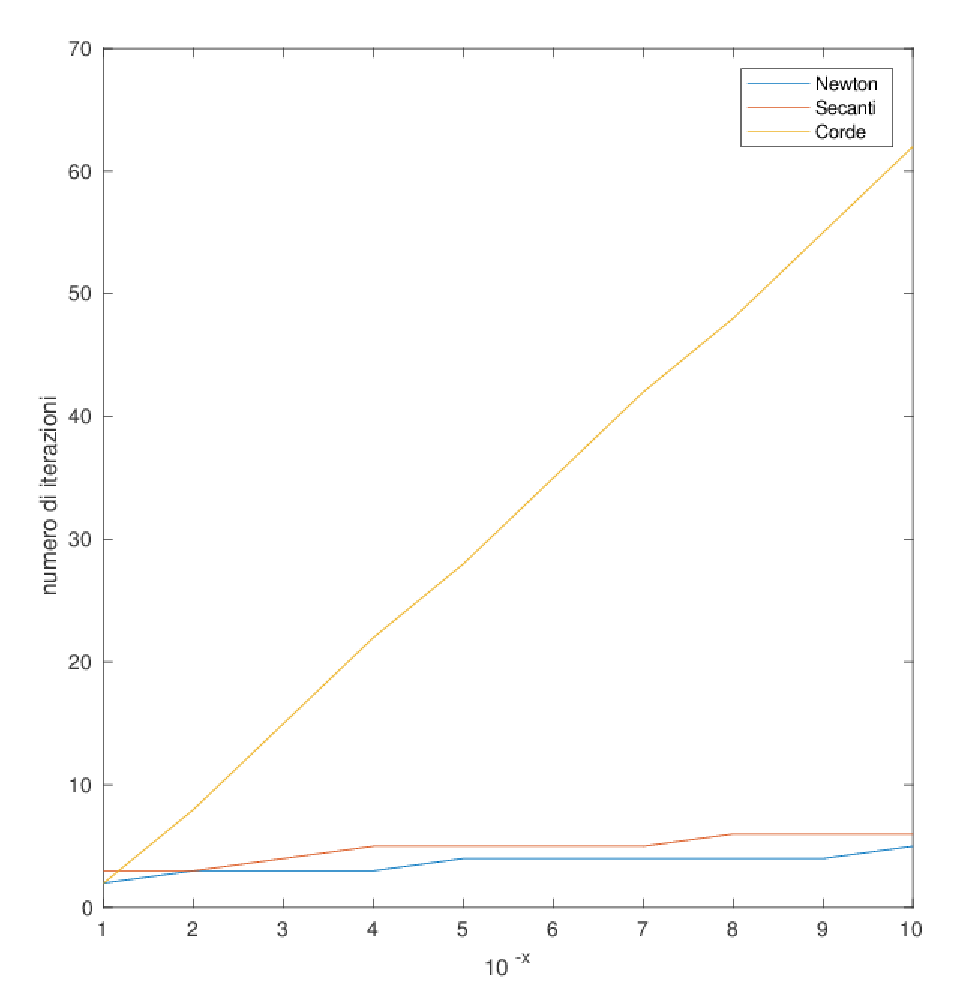
\includegraphics[width=480px, height=280px]{plot/fes26}
\caption{\texttt{\texttt{Andamento del numero delle iterazioni al decrescere della tolleranza per i metodi Newton, Secanti, Corde}}}
\end{figure}
Il numero di condizionamento del problema è dato da:
\[
k = \frac{1}{\big|f'(x^*)\big|}
\]
Per poterlo calcolare è necessario trovare la derivata della nostra funzione che è pari a:
\[
f'(x) = -1 - cos(x) + 5 \cdot sin(10\cdot x) - \frac{cos^2(10\cdot x)}{2}
\]
Essendo la radice della nostra funzione  $x^* = 0,488944$ il relativo numero di condizionamento è dato da:
\[
k = \frac{1}{\Big|f'(x^*)\Big|} = \frac{1}{\Big|f'(0,488944)\Big|} = \frac{1}{\Big|-4,27233\Big|} = \frac{1}{4,27233} = 0,234064
\]
questo significa che il problema è ben condizionato.
\end{flushleft}